\documentclass[10pt]{beamer}
\usetheme{jambro}
\graphicspath{{./graphics/}}

% Authors/institutes/date/etc
%--------------------------------
\title[]{Way Down in the Hole: Adaptation to Long-Term Water Loss in Rural India}
%\subtitle{American Economic Review}
\author[]{David Blakeslee, Ram Fishman, Veena Srinivasan}
\date{\today}

\begin{document}

%=============================================================

\begin{frame}[plain]
	\titlepage{
		\begin{center}
			\begin{minipage}{0.8\textwidth}
				\centering
				\color{title!80}{\scriptsize }
			\end{minipage}
		\end{center}}
\end{frame}

%=============================================================

\section{Introduction}
\begin{frame}
	{Introduction}
	\begin{itemize}
		\item How do rural households in India adapt to long-term water loss caused by groundwater depletion, and what role does labor reallocation to non-agricultural sectors play in maintaining household income?
		\item Data:
		      \begin{itemize}
			      \item Surveys of 1,408 households from 102 villages randomly selected in Karnataka, India
			      \item Includes: borewell failure, cropping patterns, income sources, assets, and labor reallocation
			      \item Supplemented with village-level data from the 2013 Economic Census
		      \end{itemize}
		\item Empirical strategy:
		      \begin{itemize}
			      \item Quasi-random variation from geological factors causing borewell failure as an exogenous shock
			      \item Compares households with functional borewells to those who experienced borewell failure, within villages
			      \item Household and village fixed effects
		      \end{itemize}
		\item Results:
		      \begin{itemize}
			      \item Significant drops in farm income with little evidence of agricultural adaptation
			      \item Households shifted labor to off-farm employment to offset income losses; better outcomes in regions with developed manufacturing sectors
			      \item Total income maintained through employment shifts; increased debt and asset liquidation
			      \item Older children more likely to drop out of school to supplement household income
			      \item Younger children's enrollment increased as potential preparation for future non-agricultural jobs
		      \end{itemize}
	\end{itemize}
\end{frame}

%=============================================================
\begin{frame}
	{Introduction}
	\begin{figure}
		\centering
		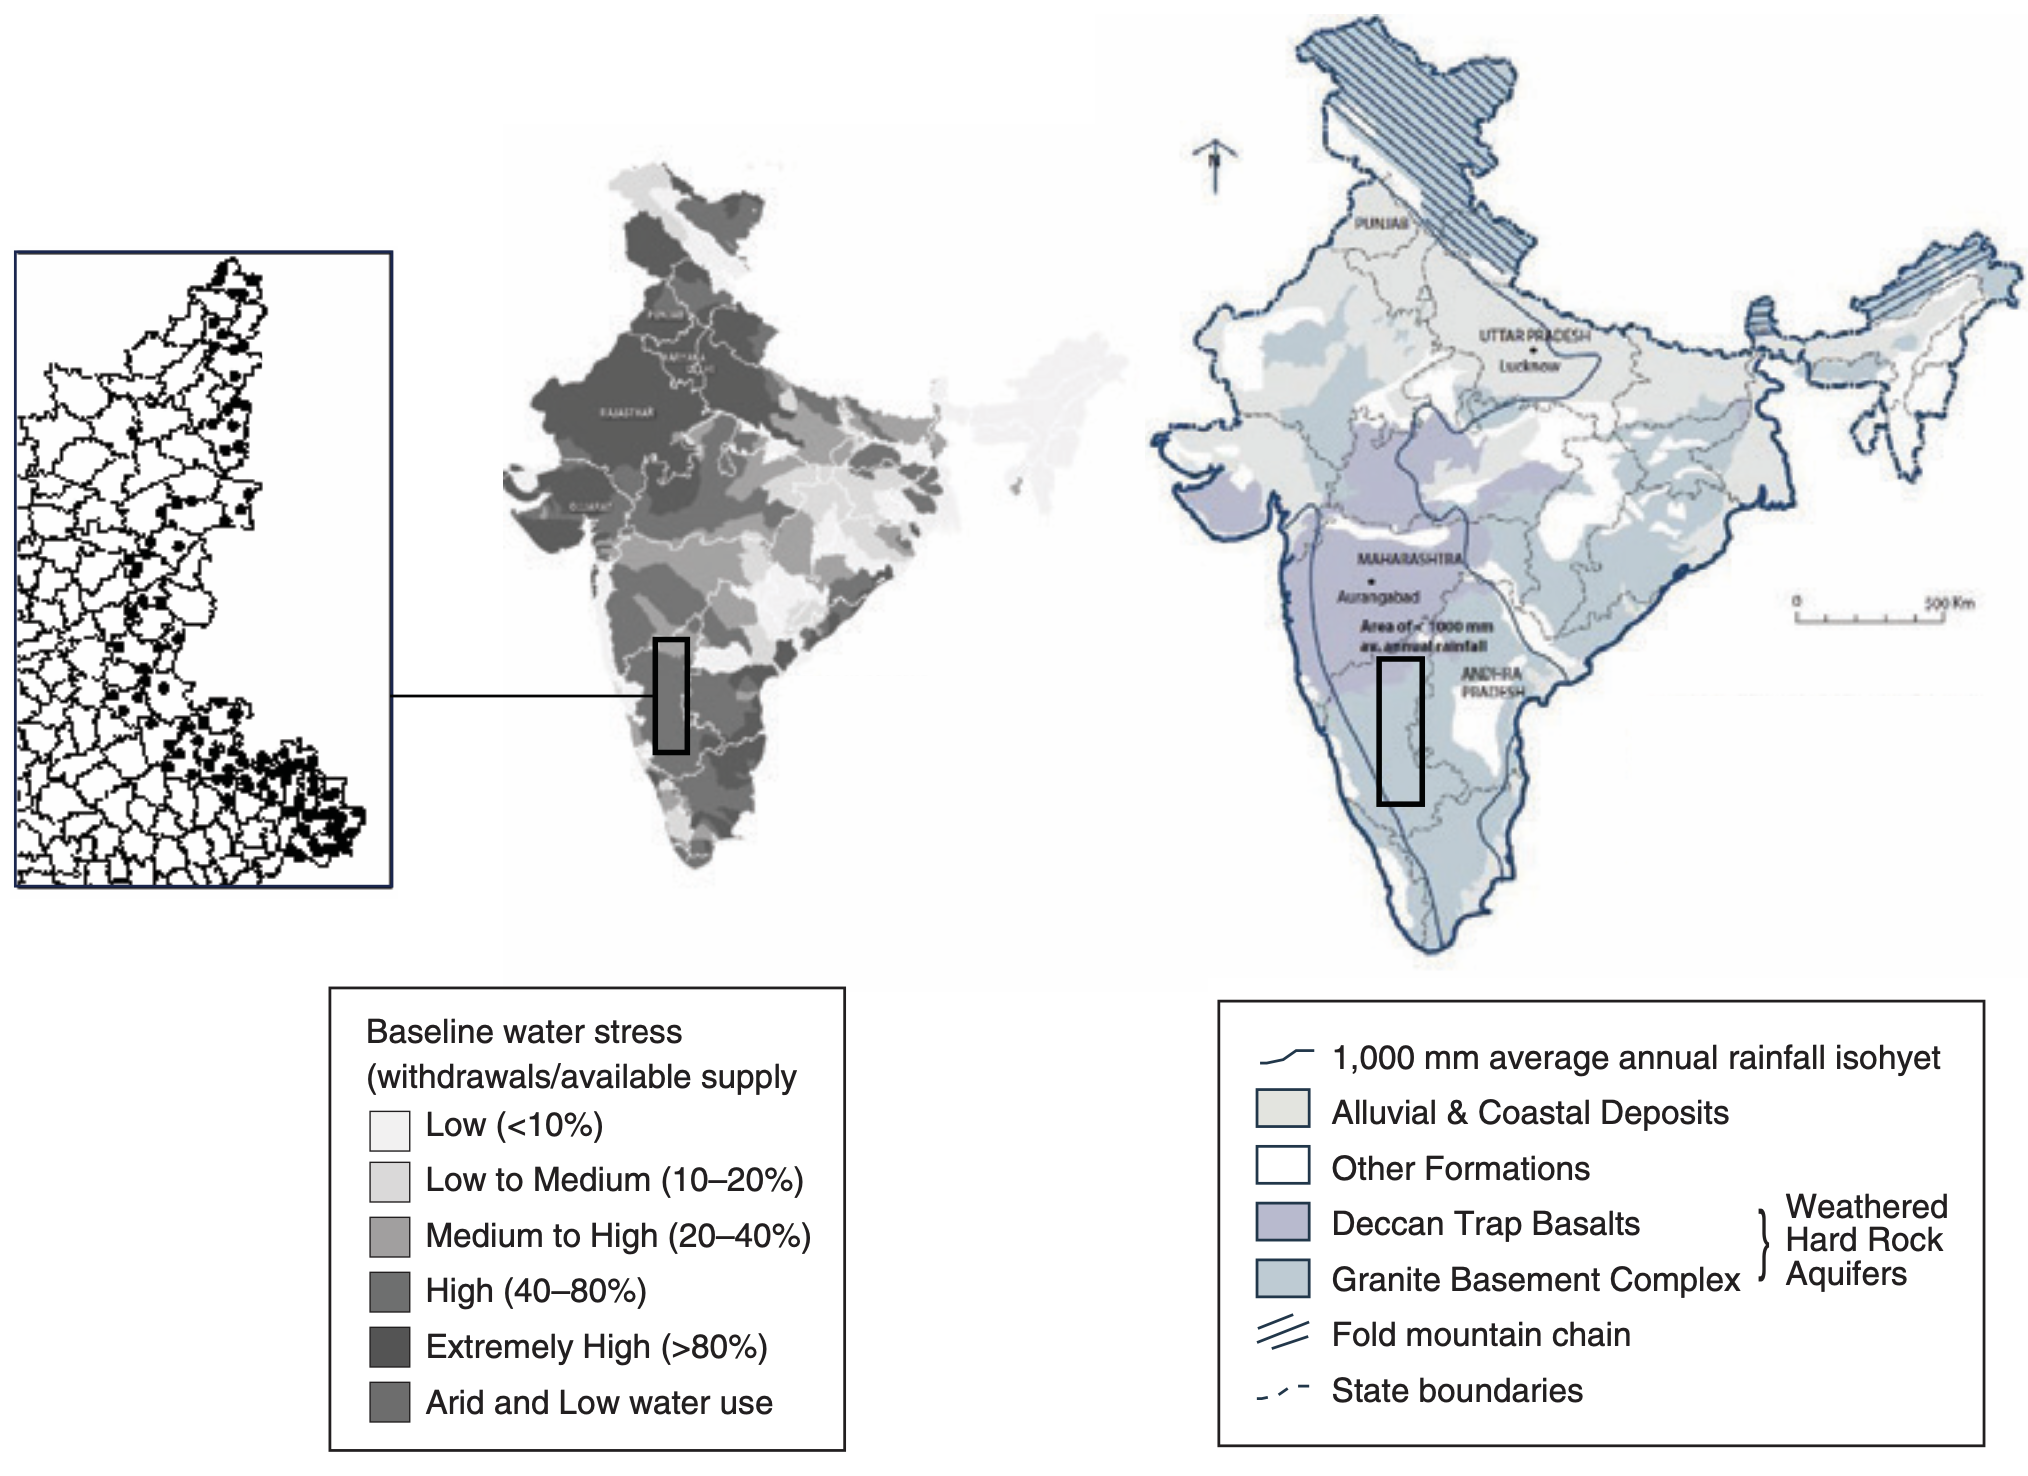
\includegraphics[width=0.55\textwidth]{figure1.png}
		\caption{Right: classification of major aquifer systems; light grey shades mark alluvial aquifers, else: hard-rock aquifers. Left: baseline water stress (withdrawals/available supply). Boxes: study area.}
	\end{figure}
\end{frame}

%=============================================================

\section{Literature Review}
\begin{frame}
	{Literature Review}
	\begin{itemize}
		\item Severe detrimental effects of climate change on agricultural livelihoods and a host of social outcomes
		      \begin{itemize}
			      \item Auffhammer et al. 2013
			      \item Dell, Jones, and Olken 2014
			      \item Carleton and Hsiang 2016
		      \end{itemize}
		\item Households' coping strategies in response to such transient income shocks, including asset sales, income diversification, and migration
		      \begin{itemize}
			      \item Alderman and Paxson 1994
			      \item Morduch 1995
			      \item Dercon 2002
		      \end{itemize}
		\item Shifts to non-agricultural employment in response to transient weather shocks
		      \begin{itemize}
			      \item Kochar 1999
			      \item Macours, Premand, and Vakis 2012
			      \item Colmer 2016
		      \end{itemize}
		\item Conceptual limitations inherent in the use of transient, high-frequency environmental variation for the purpose of studying the impacts of long-term environmental shifts
		      \begin{itemize}
			      \item Dell, Jones, and Olken 2014
			      \item Hsiang, 2016
			      \item Carleton and Hsiang 2016
		      \end{itemize}
	\end{itemize}
\end{frame}

%=============================================================

\section{Identification Strategy}
\begin{frame}
	{Identification Strategy}
	\begin{itemize}
		\item Regression:
	\end{itemize}
	\begin{equation}
		y_{i,v} = \alpha_1 + \underbrace{\alpha_2 F_i}_{\text{effect of borewell failure}} + \underbrace{X_i \Phi}_{\text{household characteristics}} + \underbrace{A_v}_{\text{village fixed effects}} + \underbrace{B_t}_{\text{year fixed effects}} + u_i
	\end{equation}
	\begin{itemize}
		\item Household characteristics include age, caste, literacy of HH head, total land inherited by HH
		\item Robustness tests: depth and cost of the first borewell, alternative specs of first borewell age
		\item All regressions incorporate sampling weights that reflect the relative share of HH in the village that belong to each type (with/without first borewell)
		\item Identifying assumption: conditional on year of drilling, failure of first borewell is exogenous, within villages, to any other correlates of the outcomes
		\item Hypothesis: remaining determinants of failure primarily depend on highly variable and quasi-random hydrogeological characteristics (such as number of sources the well intersects)
	\end{itemize}
\end{frame}


%=============================================================
\section{Results}
\begin{frame}
	{Results}
\end{frame}

%=============================================================
\section{Conclusion}

\begin{frame}
	{Conclusion}
\end{frame}

%=============================================================
\section{Thesis}
\begin{frame}
	{Thesis}
	\begin{itemize}
		\item Micro Irrigation (drip and sprinkler systems) can improve agricultural efficiency by saving 30—70 percent of water compared to conventional methods
		\item Adoption levels remain low in India due to a lack of incentives for efficiency; water and electricity is unpriced or heavily subsidized
		\item All-India Data Set: Village-level panel data from the Minor Irrigation Census (1993—2017) is used to assess adoption patterns and water scarcity correlations, merging this information with climatic data, socio-economic indicators, and satellite-based irrigation estimates
		\item Gujarat Data Set: High-resolution data from Gujarat-based GGRC tracks more than 400,000 geo-referenced MI adopters (2006—2013) and includes detailed subsidy variations, enabling analysis of adoption determinants, social learning effects, and water conservation outcomes
	\end{itemize}
\end{frame}

%=============================================================

\begin{frame}
	{Thesis}
	\begin{itemize}
		\item Working Hypotheses:
		      \begin{enumerate}
			      \item Adoption rates are correlated, across villages and farmers, with indicators of economic development and water scarcity, and these correlations are higher at early stages of diffusion. Earlier adopters are larger farmers, but MI diffuses to smaller farmers in the village over time.
			      \item Variation in water scarcity has causal impacts on the rate of adoption.
			      \item Variation in (subsidy driven) MI cost has causal impacts on the rate of adoption and particularly by smaller farmers.
			      \item Subsidized adoption has spillover effects on adoption in adjacent areas (presumably through social learning), but these are limited by crop type and social groups (castes).
			      \item Subsidized adoption has varying effects on water and power use for pumping, depending on the extent of overall irrigation coverage in the village and the existence of informal water markets.
		      \end{enumerate}
	\end{itemize}
\end{frame}


%=============================================================

\end{document}


